\begin{minipage}[t]{180mm}
\fcolorbox{black}{white}{
\begin{minipage}[b]{30mm}

\includegraphics[width=0.5\linewidth]{unflogo.pdf}
\end{minipage}
\begin{minipage}[b]{100mm}
\Huge \textbf{UNF NEWZ} \\
\Large -- Søvn og retsstavning er overvurderet! 
\end{minipage}
\begin{minipage}[b]{50mm}
\Large Onsdag 17.07.2015 \\
\normalsize Redigeret i \LaTeX\ af \\ SOM, MGS, MMN, SABH
\end{minipage}
}
\end{minipage}



\begin{minipage}[b]{0.95\linewidth}
\begin{minipage}[t]{0.47\textwidth}
\vspace{3mm}
\section*{Ninjas dagbog}
Jeg kommer til at vide, at denne dag, ikke var den bedste i mit liv. Jeg vil være blevet vækket af marcherende militærstøvler i de nordnorske bjerge, og efter lang og indædt kamp overmandet i en gammel lappehytte, af elitestyrker med kajserlige traditioner.

Kort efter vil jeg være blevet bortført sammen med storesøster og min tynde tvilling. Jeg vil være blevet bragt til et osende fly, og fløjet sydpå til skrigenes by og videre til stedet ingenører sidder i rundkreds og stønner. Op på en lastvogn af tysk mærke vil vi være blevet smidt og mod syd fragtet i høj fart.

Pludseligt i det midtjydske vil vores familiebånd hendfalde under skruebrækkernes strålekanon, og mens hydroxiden, og dermed min arvepart til sæteren, forsvandt mod undergangen i Preussernes varetægt, vil jeg, ensom og alene, sidde på en jysk bakketop.

Senere på dagen vil jeg have søgt tilflugt i de gule tårne blandt ånder som ej kendte mine evner og ej frygtede mit dræbende blik. Åndernes antal vil være blevet øget mens timerne gik, fremkaldende minder om hengangne møder på toppen af Mons Ruptus.

Førræderen over alle forræderes gudeforladte arvinger vil ydmygt have ofret os næring, og jeg vil være indgået en uhellig alliance med åndernes overhyrde og hans unge vassal. Nu selv blevet en stikker, følende knusende skyld hvor min afsavn burde have været, vil jeg have strækket min dræbende hånd ud efter almagt, og målrettet stile mod udslettelse af alle ormene jeg vil græmme mig ved.

Snart dagen vil være gået på hæld, og mens jeg vil være faldet i søvn vi jeg have hørt syngende vers, der er en sejlende quisling værdig, og minder mig og vindens faretruende susen jeg hørte i de norske højmarker på frugtbarhedens dag, som for mig varslede død frem for liv.

{\flushright\emph{Ninja, ensom og univalent}}

\end{minipage}%
\hfill\begin{minipage}[t]{0.47\textwidth}
\vspace{3mm}
\section*{Vejrudsigt}
\textbf{IMF, AU (fra DMI)}: Skyer, men med synlig sol. Op til 18 grader om dagen og ned til 12 grader om natten, ingen regn.

\textbf{IMF, AU år 2003}: Tør med dagstemperaturer op til 26 grader og nattemperaturer ned til 8 grader, 14 timers sol og næsten skyfri himmel.

\section*{Fakt om Jylland}
Jylland er ikke verdens største ø

\section*{Dagens sandsynlighed}
Sandsynligheden for at din hjerne indeholder et atom der indgik i en dinosaur er cirka $1$.

\section*{Find en Fynbo}
Rygtet siger at der har sneget sig en Fynbo ind i dette ærkejydske blad. Dette kan selvfølgelig ikke accepteres, og halvsvenskeren må derfor opspores og udraderes.

\section*{Dagens datalog}
Hvis du møder en datalog, prik ham og påpeg at der er en syntaxfejl i whitespackoden i hans blanke blik.

\section*{Ordforklaring: Whitespace}
\vspace{4cm}
\end{minipage}

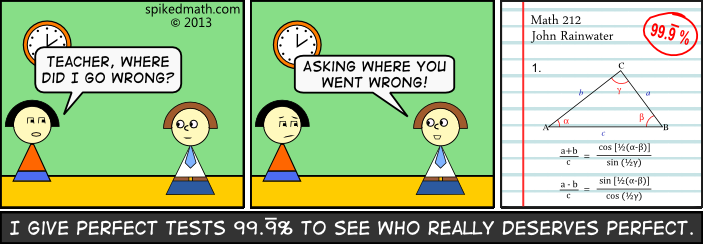
\includegraphics[width=\textwidth]{547-the-perfect-score.png}
\begin{center}
\tiny Mike, http://http://spikedmath.com/547.html, CC-BY-NC-2.5

\vspace{3mm}

\tiny UNF Newz er avisen hvor at ansvarshavende redaktør fralægger sig ethvert ansvar for enventuel plagium, kaninner, tysk, stavefelj, kaffe, dårlig humor, glemsomhed, katte, store sigmaer, pile, skyer, dårlige oversættelser og alt hvad eventuelle homosapions kunne finde på at holde imod UNF Newz! Dog tager UNF Newz fuld credit og copiright for alle guldkorn, magic kort, mus, TeX, humor, smil, mortener, kaffe, før-fremtid, ringe og/eller rubik's cube.
\end{center}
\end{minipage}

